\documentclass{beamer}
% \usetheme{metropolis}

\usepackage{../macros}
\usepackage{graphicx}
\usepackage{tikz}
\usepackage{caption}
\usepackage{adjustbox}
\usepackage{listings}
\usepackage{wrapfig}
\usepackage{color}
\usepackage{listings}
\usepackage{pgfpages}
\usepackage{msc}
\usepackage[utf8]{inputenc}
\usepackage[british]{babel}
\usepackage{amsmath}
% \setbeameroption{show notes on second screen=right}

\usetikzlibrary{automata,arrows,positioning,shapes,snakes}
\usetikzlibrary{calc,matrix,decorations.pathmorphing}
\usetikzlibrary{shapes.geometric,arrows.meta}
\pgfmathtruncatemacro\distance{1}

\addtobeamertemplate{navigation symbols}{}{%
    \usebeamerfont{footline}%
    \usebeamercolor[fg]{footline}%
    \hspace{1em}%
    \insertframenumber/\inserttotalframenumber
}

\setbeamercolor{footline}{fg=blue}
\setbeamerfont{footline}{series=\bfseries}

\tikzset{
    mylabel/.style={
    font=\tiny,
    sloped,
    above
  }
}

\lstset{language=erlang, basicstyle=\sffamily\footnotesize,
  keywordstyle=\color{blue}, numberstyle=\tiny, numbers=none,
  showspaces=false, showstringspaces=false, frame=tL, mathescape=true,
  backgroundcolor=\color{black!5}, morekeywords={send, to, from} }


\title{Realisability of Global Types:\\Decidability and Verification}
% \author{
% 	\textbf{Presentata da: Gabriele Genovese},
% 	Relatore: Prof. Ivan Lanese,
% 	Corelatori: Prof. Cinzia Di Giusto e Chiar.mo Prof. Étienne Lozes,
% 	Controrelatore: Chiar.mo Prof. Luca Padovani
% 	}
\author[Gabriele Genovese]{Presentata da: \textbf{Gabriele Genovese}\\[4mm]{\small 
	Relatore: Prof. Ivan Lanese \\ 
	\hspace{2.4mm} Correlatori: Prof. Cinzia Di Giusto \\ \hspace{30.8mm} Chiar.mo Prof. Étienne Lozes \\
	\hspace{8.8mm} Controrelatore: Chiar.mo Prof. Luca Padovani}
}
\date{30 Ottobre 2025}

\titlegraphic{
\includegraphics[width=2cm]{../img/i3s.png}\hspace*{4.75cm}~%
   
\includegraphics[width=1.4cm]{../img/logo.png}
}


\begin{document}

\maketitle
\note{
	Good morning, everyone. I'm Gabriele Genovese.
}


\begin{frame}{Multiparty Session Types}
	\begin{itemize}
		\item Honda, K., Yoshida, N., and Carbone, M. (2008)
		\item Verification and design of \emph{communication protocols} 
		\item Avoid \emph{deadlocks}, ensure \emph{progress}, etc...
	\end{itemize}

	\begin{center}
	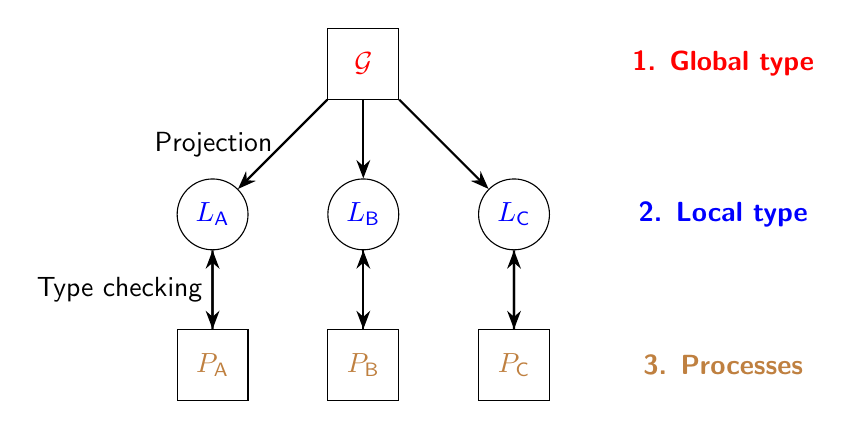
\begin{tikzpicture}[
		node distance=1cm,
		every node/.style={font=\sffamily},
		rect/.style={rectangle, draw=black, minimum width=0.9cm, minimum height=0.9cm},
		circ/.style={circle, draw=black, minimum size=0.9cm},
		arrow/.style={-{Stealth}, thick}, scale=0.1
	]

	% Nodes
	\node[rect] (G) {\textcolor{red}{$\mathcal{G}$}};
	\node[circ, below=of G] (TB) {\textcolor{blue}{$L_\text{B}$}};
	\node[circ, left=of TB] (TA) {\textcolor{blue}{$L_\text{A}$}};
	\node[circ, right=of TB] (TC) {\textcolor{blue}{$L_\text{C}$}};

	\node[rect, below=of TA] (PA) {\textcolor{brown}{$P_\text{A}$}};
	\node[rect, below=of TB] (PB) {\textcolor{brown}{$P_\text{B}$}};
	\node[rect, below=of TC] (PC) {\textcolor{brown}{$P_\text{C}$}};

	\node[rect,draw=none,right=of TC] (LC) {\textbf{\textcolor{blue}{2. Local type}}};
	\node[rect,draw=none,above=of LC] (LG) {\textbf{\textcolor{red}{1. Global type}}};
	\node[rect,draw=none,below=of LC] (LG) {\textbf{\textcolor{brown}{3. Processes}}};

	% Arrows
	\draw[arrow] (G) -- (TA) node[midway, left] {Projection};
	\draw[arrow] (G) -- (TB);
	\draw[arrow] (G) -- (TC);

	\draw[arrow] (PA) -- (TA) node[midway, left] {Type checking};
	\draw[arrow] (PB) -- (TB);
	\draw[arrow] (PC) -- (TC);
	\draw[arrow] (TC) -- (PC);
	\draw[arrow] (TB) -- (PB);
	\draw[arrow] (TA) -- (PA);

	\end{tikzpicture}
	\end{center}
\end{frame}


\tikzstyle{box} = [rectangle, rounded corners, draw=blue!60, fill=blue!10, thick,
text width=7.5em, text centered, minimum height=2em]


% \newcommand{\marrow}[3]{#1\xrightarrow{#3}#2}
% \newcommand{\gtlabel}[3]{\marrow{#1}{#2}{#3}}
\begin{frame}{Global Types}
	\begin{itemize}
		\item Description of a \textbf{global} behavior of a system.
		\item Defined as automata
	\end{itemize}

	\bigskip

	\begin{center}
		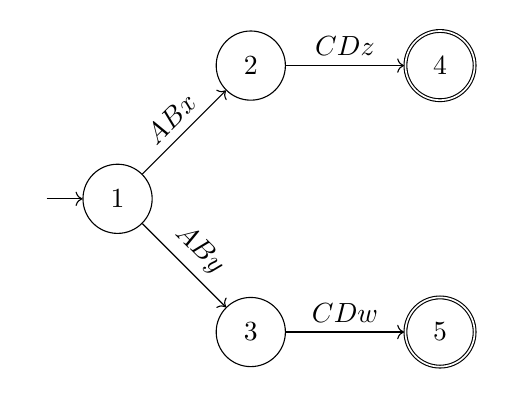
\begin{tikzpicture}[node distance=1.5cm, auto]
			\node[state, initial, initial text={}] (s0) {1};
			\node[state] (s1) [above right=of s0] {2};
			\node[state] (s2) [below right=of s0] {3};
			\node[state,accepting] (s3) [right=of s1] {4};
			\node[state,accepting] (s4) [right=of s2] {5};

			\draw[->] (s0) to node[above,sloped]{$\gtlabel{A}{B}{x}$}(s1);
			\draw[->] (s0) to node[above,sloped]{$\gtlabel{A}{B}{y}$}(s2);
			\draw[->] (s1) to node[above,sloped]{$\gtlabel{C}{D}{z}$}(s3);
			\draw[->] (s2) to node[above,sloped]{$\gtlabel{C}{D}{w}$}(s4);

		\end{tikzpicture}
	\end{center}
\end{frame}

\begin{frame}{Local type}
	\begin{itemize}
		\item Point of view of a participant
		\item Obtained via \textit{projection} operation
		\item Behavior can differ for different communication semantics (p2p, sync) 
	\end{itemize}

	\bigskip

	\textbf{Realisability} problem: Does the implementation of a system 
  \textbf{respects} the behavior described?

	\bigskip

	$L(G) = L(\text{proj}(G))$

	% \begin{center}
	% 	\begin{tikzpicture}[node distance=3cm, auto]
	% 		\node[state, initial, initial text={}] (s0) {$s_0$};
	% 		\node[state] (s1) [right=of s0] {$s_1$};
	% 		\node[state,accepting] (s2) [right=of s1] {$s_2$};

	% 		\draw[->] (s0) -- node[above,sloped]{$A!B:ping$} (s1);
	% 		\draw[->] (s1) -- node[above,sloped]{$A?B:pong$} (s2);
	% 	\end{tikzpicture}
	% \end{center}

	% \begin{center}
	% 	\begin{tikzpicture}[node distance=3cm, auto]
	% 		\node[state, initial, initial text={}] (s0) {$s_0$};
	% 		\node[state] (s1) [right=of s0] {$s_1$};
	% 		\node[state,accepting] (s2) [right=of s1] {$s_2$};

	% 		\draw[->] (s0) -- node[above,sloped]{$B?A:ping$} (s1);
	% 		\draw[->] (s1) -- node[above,sloped]{$B!A:pong$} (s2);
	% 	\end{tikzpicture}
	% \end{center}
\end{frame}

% \begin{frame}{Example}
% 	Message Queuing Telemetry Transport (MQTT) protocol with two clients.
% 	\begin{center}
% 		\begin{tikzpicture}[node distance=3cm, auto]
% 			\node[state, initial, initial text={}] (s0) {$s_0$};
% 			\node[state] (s1) [above right=of s0] {$s_1$};
% 			\node[state] (s2) [right=of s0] {$s_2$};

% 			\draw[->, bend left=40] (s0) to node[above,sloped]{$\gtlabel{C_1}{B}{pub(m)}$}(s1);
% 			\draw[->] (s1) to node[above,sloped] {$\gtlabel{B}{C_2}{pub(m)}$} (s0);

% 			\draw[->, bend left=20] (s0) to node[above,sloped]{$\gtlabel{C_2}{B}{pub(m)}$}(s2);
% 			\draw[->] (s2) -- node[below,sloped]{$\gtlabel{B}{C_1}{pub(m)}$} (s0);
% 		\end{tikzpicture}
% 	\end{center}
% \end{frame}


\begin{frame}{The example is not realisable}
	This example is {\color{red}\textbf{not}} realisable 
	because $C$ doesn't know what $A$ sent.
	\begin{center}
		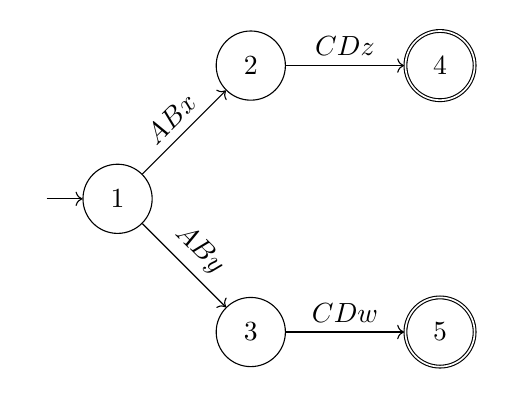
\begin{tikzpicture}[node distance=1.5cm, auto]
			\node[state, initial, initial text={}] (s0) {1};
			\node[state] (s1) [above right=of s0] {2};
			\node[state] (s2) [below right=of s0] {3};
			\node[state,accepting] (s3) [right=of s1] {4};
			\node[state,accepting] (s4) [right=of s2] {5};

			\draw[->] (s0) to node[above,sloped]{$\gtlabel{A}{B}{x}$}(s1);
			\draw[->] (s0) to node[above,sloped]{$\gtlabel{A}{B}{y}$}(s2);
			\draw[->] (s1) to node[above,sloped]{$\gtlabel{C}{D}{z}$}(s3);
			\draw[->] (s2) to node[above,sloped]{$\gtlabel{C}{D}{w}$}(s4);

		\end{tikzpicture}
	\end{center}

	The trace $\gtlabel{A}{B}{x};\gtlabel{C}{D}{w}$ does not appear in $L(G)$.
\end{frame}

% \begin{frame}[fragile]{Message Sequence Charts (MSC)}
% 	Diagrams used to represent traces of a behavior of the system.

% 	\bigskip

% 	% \hspace{-2em}
% 	\begin{minipage}{\textwidth}%0.45\textwidth}
% 		\centering
% 		\begin{msc}[draw frame=none, draw head=none, msc keyword=, head height=0px, label distance=0.5ex, foot height=0px, foot distance=0px]{}
% 			\declinst{P1}{P1}{}
% 			\declinst{P2}{P2}{}
% 			\declinst{P3}{P3}{}

% 			\asyncmscmess{$m_1$}{P1}{P2}
% 			\asyncmscmess{$m_2$}{P2}{P3}
% 		\end{msc}
% 	\end{minipage}
% 	% \hspace{0.1\textwidth}
% 	% \begin{minipage}{0.45\textwidth}
% 	% 	\centering
% 	% 	\begin{msc}[draw frame=none, draw head=none, msc keyword=, head height=0px, label distance=0.5ex, foot height=0px, foot distance=0px]{}
% 	% 		\declinst{P1}{P1}{}
% 	% 		\declinst{P2}{P2}{}

% 	% 		\mess{$m_1$}{P1}{P2}[1]
% 	% 		\mess{$m_2$}{P2}{P1}[3]
% 	% 	\end{msc}
% 	% \end{minipage}
% 	% descrive gli eventi send and receive
% 	\begin{center}
% 		Events: \verb|send m1, receive m1, send m2, receive m2|
% 	\end{center}
% \end{frame}

% \begin{frame}{Communication models}
% 	More interesting: async, p2p, mb (mailbox), rsc (sync).

% \end{frame}

\begin{frame}{Reduction to sync [1]}
	\vspace{1.5cm}
	A global type $G$ is deadlock-free realisable in \textbf{p2p} iff:
	\begin{enumerate}
		\item $L_{\text{p2p}}(proj(G))$ is sync;
		\item $proj(G)$ is orphan-free in p2p; % (no message is sent but not received)
		\item $L_{\text{p2p}}(proj(G))$ is deadlock-free
		\item $G$ is weak realisable in sync
		\item $G$ is deadlock-free in sync
	\end{enumerate}
	
	\vspace{1.5cm}

	\small{[1] Di Giusto, Cinzia, Etienne Lozes, and Pascal Urso. "Realisability and Complementability of Multiparty Session Types." (2025).}
\end{frame}

\begin{frame}{Reduction to sync [1]}
	\vspace{1.5cm}
	A global type $G$ is deadlock-free realisable in \textbf{p2p} iff:
	\begin{enumerate}
		\item $L_{\text{p2p}}(proj(G))$ is sync;
		\item $proj(G)$ is orphan-free in p2p; % (no message is sent but not received)
		\item $L_{\text{p2p}}(proj(G))$ is deadlock-free
		\item $G$ is weak realisable in sync \hspace{4mm} \scalebox{1.5}{{\color{red}$\longleftarrow$}}
		\item $G$ is deadlock-free in sync 
	\end{enumerate}
	
	\vspace{1.5cm}

	\small{[1] Di Giusto, Cinzia, Etienne Lozes, and Pascal Urso. "Realisability and Complementability of Multiparty Session Types." (2025).}
\end{frame}

\begin{frame}[fragile]{First contribution}

	\vspace{1em}

	\begin{itemize}
		\item Realisability for sync global types is
    \textbf{undecidable}. \\ Proof: by reduction to the PCP problem.
    \item PCP:Given a set of tiles, find an ordering such that the
    strings formed by the top and bottom halves are equal.
    \item Proof adaptated from Alur et al.~[2]
	\end{itemize}

	\begin{center}
		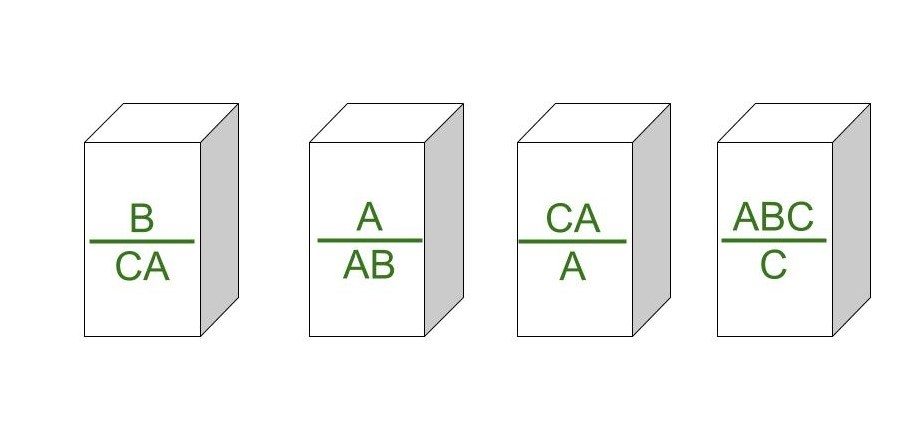
\includegraphics[width=0.6\textwidth]{../img/pcp.jpg}
	\end{center}

	\small{[2] Alur, Rajeev, Kousha Etessami, and Mihalis Yannakakis. "Realizability and verification of MSC graphs." Theoretical Computer Science 331.1 (2005): 97-114.}
\end{frame}

\begin{frame}{Reduction to sync [1]}
	\vspace{1.5cm}
	A global type $G$ is deadlock-free realisable in \textbf{p2p} iff:
	\begin{enumerate}
		\item $L_{\text{p2p}}(proj(G))$ is sync;
		\item $proj(G)$ is orphan-free in p2p; % (no message is sent but not received)
		\item $L_{\text{p2p}}(proj(G))$ is deadlock-free
		\item $G$ is weak realisable in sync
		\item $G$ is deadlock-free in sync \hspace{4mm} \scalebox{1.5}{{\color{red}$\longleftarrow$}}
	\end{enumerate}
	
	\vspace{1.5cm}

	\small{[1] Di Giusto, Cinzia, Etienne Lozes, and Pascal Urso. "Realisability and Complementability of Multiparty Session Types." (2025).}
\end{frame}

\begin{frame}[fragile]{Second contribution}

	\begin{itemize}
		\item \textsc{ReSCu}: Model-checking TUI tool written in OCaml
		\bigskip
		\item Added two verification if \emph{sync} system:
		\begin{itemize}
			\item \emph{Deadlock}: a final state is always reachable
			\item \emph{Progress}: the system can always perform an action
		\end{itemize} 
	\end{itemize}
	
\end{frame}

\begin{frame}[fragile]{\textsc{ReSCu} Example - Dining Philosophers}
	Two Philosophers, two forks.

	\bigskip

	\begin{lstlisting}
This system is RSC.
There are some sink states:
Sink: Id=11 Configuration={F0:4; F1:3; P1:2; P2:2}
There are some deadlock states:
Deadlock: Id=4 Configuration={F0:2; F1:1; P1:1; P2:1}
Deadlock: Id=11 Configuration={F0:4; F1:3; P1:2; P2:2}
...
    \end{lstlisting}
\end{frame}


\begin{frame}{\textsc{ReSCu} Example - Dining Philosophers}
\begin{center}
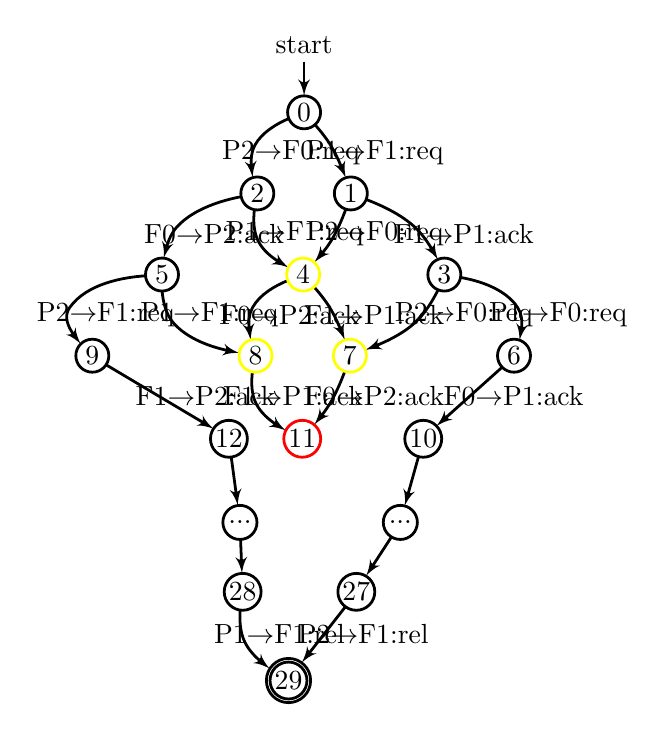
\begin{tikzpicture}[>=latex',line join=bevel,scale=0.33]
  \pgfsetlinewidth{1bp}
%%
\pgfsetcolor{black}
  % Edge: F02F10P10P21 -> F04F10P10P22
  \draw [->] (190.31bp,551.88bp) .. controls (170.67bp,548.11bp) and (139.47bp,539.27bp)  .. (120.97bp,519.48bp) .. controls (114.96bp,513.06bp) and (111.11bp,504.46bp)  .. (106.05bp,485.16bp);
  \definecolor{strokecol}{rgb}{0.0,0.0,0.0};
  \pgfsetstrokecolor{strokecol}
  \draw (161.09bp,511.23bp) node {F0$\to$P2:ack};
  % Edge: F02F10P10P21 -> F02F11P11P21
  \draw [->] (204.93bp,537.28bp) .. controls (203.79bp,526.78bp) and (203.95bp,513.42bp)  .. (209.47bp,502.98bp) .. controls (214.49bp,493.47bp) and (223.38bp,485.95bp)  .. (241.94bp,474.84bp);
  \draw (248.84bp,511.23bp) node {P1$\to$F1:req};
  % Edge: F00F11P11P20 -> F00F13P12P20
  \draw [->] (327.34bp,548.73bp) .. controls (342.31bp,543.07bp) and (363.97bp,533.26bp)  .. (379.22bp,519.48bp) .. controls (387.26bp,512.21bp) and (394.13bp,502.55bp)  .. (405.07bp,483.5bp);
  \draw (433.49bp,511.23bp) node {F1$\to$P1:ack};
  % Edge: F00F11P11P20 -> F02F11P11P21
  \draw [->] (304.68bp,538.08bp) .. controls (300.8bp,527.63bp) and (295.1bp,514.04bp)  .. (288.22bp,502.98bp) .. controls (285.26bp,498.22bp) and (281.67bp,493.44bp)  .. (270.63bp,480.53bp);
  \draw (336.25bp,511.23bp) node {P2$\to$F0:req};
  % Edge: F00F14P16P25 -> F00F10P16P26
  \draw [->] (304.33bp,104.67bp) .. controls (293.44bp,90.719bp) and (277.04bp,69.729bp)  .. (256.88bp,43.906bp);
  \draw (323.72bp,74.512bp) node {P2$\to$F1:rel};
  % Edge: F00F10P10P20 -> F02F10P10P21
  \draw [->] (242.27bp,637.06bp) .. controls (229.61bp,631.64bp) and (213.22bp,622.27bp)  .. (205.47bp,607.98bp) .. controls (201.63bp,600.89bp) and (200.83bp,592.42bp)  .. (203.04bp,573.23bp);
  \draw (244.84bp,599.73bp) node {P2$\to$F0:req};
  % Edge: F00F10P10P20 -> F00F11P11P20
  \draw [->] (271.19bp,630.36bp) .. controls (276.83bp,623.98bp) and (283.37bp,615.93bp)  .. (288.22bp,607.98bp) .. controls (292.88bp,600.33bp) and (297.04bp,591.52bp)  .. (304.61bp,572.84bp);
  \draw (336.18bp,599.73bp) node {P1$\to$F1:req};
  % Edge: F04F10P10P22 -> F04F11P11P22
  \draw [->] (104.36bp,448.85bp) .. controls (105.32bp,437.85bp) and (108.26bp,423.91bp)  .. (116.47bp,414.48bp) .. controls (131.82bp,396.84bp) and (157.16bp,388.03bp)  .. (188.23bp,381.53bp);
  \draw (155.84bp,422.73bp) node {P1$\to$F1:req};
  % Edge: F04F10P10P22 -> F04F12P10P23
  \draw [->] (85.982bp,465.61bp) .. controls (62.433bp,464.04bp) and (22.249bp,457.38bp)  .. (3.468bp,430.98bp) .. controls (-3.2418bp,421.54bp) and (1.3095bp,410.01bp)  .. (15.345bp,391.56bp);
  \draw (42.843bp,422.73bp) node {P2$\to$F1:req};
  % Edge: F04F14P10P24 -> F00F14P10P25
  \draw [->] (179.82bp,267.49bp) .. controls (181.43bp,255.51bp) and (183.53bp,239.92bp)  .. (186.82bp,215.43bp);
  % \draw (222.17bp,241.47bp) node {P2$\to$F0:rel};
  % Edge: F00F13P15P26 -> F00F10P16P26
  \draw [->] (189.41bp,100.63bp) .. controls (188.73bp,89.988bp) and (189.35bp,76.831bp)  .. (194.47bp,66.262bp) .. controls (198.56bp,57.814bp) and (205.27bp,50.41bp)  .. (221.45bp,37.266bp);
  \draw (232.34bp,74.512bp) node {P1$\to$F1:rel};
  % Edge: F00F13P12P20 -> F01F13P13P20
  \draw [->] (430.17bp,463.79bp) .. controls (449.25bp,460.4bp) and (478.53bp,451.91bp)  .. (492.22bp,430.98bp) .. controls (496.82bp,423.94bp) and (497.52bp,415.14bp)  .. (494.3bp,395.62bp);
  \draw (536.24bp,422.73bp) node {P1$\to$F0:req};
  % Edge: F00F13P12P20 -> F02F13P12P21
  \draw [->] (405.19bp,449.94bp) .. controls (399.68bp,438.85bp) and (391.14bp,424.38bp)  .. (380.22bp,414.48bp) .. controls (367.77bp,403.19bp) and (351.01bp,394.7bp)  .. (326.28bp,384.84bp);
  \draw (433.49bp,422.73bp) node {P2$\to$F0:req};
  % Edge: F02F11P11P21 -> F04F11P11P22
  \draw [->] (241.08bp,460.3bp) .. controls (228.04bp,454.97bp) and (211.02bp,445.6bp)  .. (202.97bp,430.98bp) .. controls (199.02bp,423.81bp) and (198.31bp,415.19bp)  .. (200.87bp,395.78bp);
  \draw (243.09bp,422.73bp) node {F0$\to$P2:ack};
  % Edge: F02F11P11P21 -> F02F13P12P21
  \draw [->] (270.19bp,453.36bp) .. controls (275.83bp,446.98bp) and (282.37bp,438.93bp)  .. (287.22bp,430.98bp) .. controls (291.88bp,423.33bp) and (296.04bp,414.52bp)  .. (303.61bp,395.84bp);
  \draw (335.93bp,422.73bp) node {F1$\to$P1:ack};
  % Edge: F04F11P11P22 -> F04F13P12P22
  \draw [->] (202.78bp,360.32bp) .. controls (201.54bp,349.84bp) and (201.58bp,336.48bp)  .. (206.97bp,325.98bp) .. controls (211.87bp,316.44bp) and (220.47bp,308.74bp)  .. (238.89bp,297.02bp);
  \draw (247.09bp,334.23bp) node {F1$\to$P1:ack};
  % Edge: start_node -> F00F10P10P20
  \draw [->] (259.22bp,699.15bp) .. controls (259.22bp,691.54bp) and (259.22bp,682.33bp)  .. (259.22bp,662.42bp);
  % Edge: F01F13P13P20 -> F03F13P14P20
  \draw [->] (475.28bp,365.89bp) .. controls (459.28bp,351.57bp) and (431.77bp,326.94bp)  .. (403.77bp,301.88bp);
  \draw (487.71bp,334.23bp) node {F0$\to$P1:ack};
  % Edge: F04F12P10P23 -> F04F14P10P24
  \draw [->] (43.602bp,368.33bp) .. controls (68.854bp,353.31bp) and (119.39bp,323.24bp)  .. (160.33bp,298.89bp);
  \draw (151.76bp,334.23bp) node {F1$\to$P2:ack};
  % Edge: F02F13P12P21 -> F04F13P12P22
  \draw [->] (303.57bp,361.14bp) .. controls (299.65bp,350.73bp) and (293.93bp,337.14bp)  .. (287.22bp,325.98bp) .. controls (284.38bp,321.26bp) and (280.99bp,316.48bp)  .. (270.47bp,303.33bp);
  \draw (335.87bp,334.23bp) node {F0$\to$P2:ack};
  % Edge: F03F13P14P20 -> F02F13P15P21
  \draw [->] (383.92bp,267.92bp) .. controls (380.49bp,255.69bp) and (375.97bp,239.56bp)  .. (369.09bp,215.0bp);
  % Edge: F00F14P10P25 -> F00F13P15P26
  \draw [->] (189.94bp,177.77bp) .. controls (190.25bp,170.21bp) and (190.62bp,161.19bp)  .. (191.42bp,141.39bp);
  % Edge: F02F13P15P21 -> F00F14P16P25
  \draw [->] (354.27bp,180.34bp) .. controls (348.18bp,170.98bp) and (340.21bp,158.74bp)  .. (326.99bp,138.43bp);
  % Node: F02F10P10P21
\begin{scope}
  \definecolor{strokecol}{rgb}{0.0,0.0,0.0};
  \pgfsetstrokecolor{strokecol}
  \draw (208.22bp,555.48bp) ellipse (18.0bp and 18.0bp);
  \draw (208.22bp,555.48bp) node {2};
\end{scope}
  % Node: F04F10P10P22
\begin{scope}
  \definecolor{strokecol}{rgb}{0.0,0.0,0.0};
  \pgfsetstrokecolor{strokecol}
  \draw (104.22bp,466.98bp) ellipse (18.0bp and 18.0bp);
  \draw (104.22bp,466.98bp) node {5};
\end{scope}
  % Node: F02F11P11P21
\begin{scope}
  \definecolor{strokecol}{rgb}{1.0,1.0,0.0};
  \pgfsetstrokecolor{strokecol}
  \draw (258.22bp,466.98bp) ellipse (18.0bp and 18.0bp);
  \definecolor{strokecol}{rgb}{0.0,0.0,0.0};
  \pgfsetstrokecolor{strokecol}
  \draw (258.22bp,466.98bp) node {4};
\end{scope}
  % Node: F00F11P11P20
\begin{scope}
  \definecolor{strokecol}{rgb}{0.0,0.0,0.0};
  \pgfsetstrokecolor{strokecol}
  \draw (310.22bp,555.48bp) ellipse (18.0bp and 18.0bp);
  \draw (310.22bp,555.48bp) node {1};
\end{scope}
  % Node: F00F13P12P20
\begin{scope}
  \definecolor{strokecol}{rgb}{0.0,0.0,0.0};
  \pgfsetstrokecolor{strokecol}
  \draw (412.22bp,466.98bp) ellipse (18.0bp and 18.0bp);
  \draw (412.22bp,466.98bp) node {3};
\end{scope}
  % Node: F00F14P16P25
\begin{scope}
  \definecolor{strokecol}{rgb}{0.0,0.0,0.0};
  \pgfsetstrokecolor{strokecol}
  \draw (316.22bp,120.89bp) ellipse (20.13bp and 20.13bp);
  \draw (316.22bp,120.89bp) node {27};
\end{scope}
  % Node: F00F10P16P26
\begin{scope}
  \definecolor{strokecol}{rgb}{0.0,0.0,0.0};
  \pgfsetstrokecolor{strokecol}
  \draw (242.22bp,24.13bp) ellipse (20.13bp and 20.13bp);
  \draw (242.22bp,24.13bp) ellipse (24.13bp and 24.13bp);
  \draw (242.22bp,24.131bp) node {29};
\end{scope}
  % Node: F00F10P10P20
\begin{scope}
  \definecolor{strokecol}{rgb}{0.0,0.0,0.0};
  \pgfsetstrokecolor{strokecol}
  \draw (259.22bp,643.98bp) ellipse (18.0bp and 18.0bp);
  \draw (259.22bp,643.98bp) node {0};
\end{scope}
  % Node: F04F11P11P22
\begin{scope}
  \definecolor{strokecol}{rgb}{1.0,1.0,0.0};
  \pgfsetstrokecolor{strokecol}
  \draw (206.22bp,378.48bp) ellipse (18.0bp and 18.0bp);
  \definecolor{strokecol}{rgb}{0.0,0.0,0.0};
  \pgfsetstrokecolor{strokecol}
  \draw (206.22bp,378.48bp) node {8};
\end{scope}
  % Node: F04F12P10P23
\begin{scope}
  \definecolor{strokecol}{rgb}{0.0,0.0,0.0};
  \pgfsetstrokecolor{strokecol}
  \draw (28.22bp,378.48bp) ellipse (18.0bp and 18.0bp);
  \draw (28.218bp,378.48bp) node {9};
\end{scope}
  % Node: F04F14P10P24
\begin{scope}
  \definecolor{strokecol}{rgb}{0.0,0.0,0.0};
  \pgfsetstrokecolor{strokecol}
  \draw (177.22bp,287.85bp) ellipse (20.13bp and 20.13bp);
  \draw (177.22bp,287.85bp) node {12};
\end{scope}
  % Node: F00F14P10P25
\begin{scope}
  \definecolor{strokecol}{rgb}{0.0,0.0,0.0};
  \pgfsetstrokecolor{strokecol}
  \draw (189.22bp,196.62bp) ellipse (18.6bp and 18.6bp);
  \draw (189.22bp,196.62bp) node {...};
\end{scope}
  % Node: F00F13P15P26
\begin{scope}
  \definecolor{strokecol}{rgb}{0.0,0.0,0.0};
  \pgfsetstrokecolor{strokecol}
  \draw (192.22bp,120.89bp) ellipse (20.13bp and 20.13bp);
  \draw (192.22bp,120.89bp) node {28};
\end{scope}
  % Node: F01F13P13P20
\begin{scope}
  \definecolor{strokecol}{rgb}{0.0,0.0,0.0};
  \pgfsetstrokecolor{strokecol}
  \draw (488.22bp,378.48bp) ellipse (18.0bp and 18.0bp);
  \draw (488.22bp,378.48bp) node {6};
\end{scope}
  % Node: F02F13P12P21
\begin{scope}
  \definecolor{strokecol}{rgb}{1.0,1.0,0.0};
  \pgfsetstrokecolor{strokecol}
  \draw (309.22bp,378.48bp) ellipse (18.0bp and 18.0bp);
  \definecolor{strokecol}{rgb}{0.0,0.0,0.0};
  \pgfsetstrokecolor{strokecol}
  \draw (309.22bp,378.48bp) node {7};
\end{scope}
  % Node: F04F13P12P22
\begin{scope}
  \definecolor{strokecol}{rgb}{1.0,0.0,0.0};
  \pgfsetstrokecolor{strokecol}
  \draw (257.22bp,287.85bp) ellipse (20.13bp and 20.13bp);
  \definecolor{strokecol}{rgb}{0.0,0.0,0.0};
  \pgfsetstrokecolor{strokecol}
  \draw (257.22bp,287.85bp) node {11};
\end{scope}
  % Node: start_node
\begin{scope}
  \definecolor{strokecol}{rgb}{0.0,0.0,0.0};
  \pgfsetstrokecolor{strokecol}
  \draw (259.22bp,716.98bp) node {start};
\end{scope}
  % Node: F03F13P14P20
\begin{scope}
  \definecolor{strokecol}{rgb}{0.0,0.0,0.0};
  \pgfsetstrokecolor{strokecol}
  \draw (389.22bp,287.85bp) ellipse (20.13bp and 20.13bp);
  \draw (389.22bp,287.85bp) node {10};
\end{scope}
  % Node: F02F13P15P21
\begin{scope}
  \definecolor{strokecol}{rgb}{0.0,0.0,0.0};
  \pgfsetstrokecolor{strokecol}
  \draw (364.22bp,196.62bp) ellipse (18.6bp and 18.6bp);
  \draw (364.22bp,196.62bp) node {...};
\end{scope}
%
\end{tikzpicture}
\end{center}
\end{frame}



% \begin{frame}{State of the art}
% 	The study about implementability can be summarized in:

% 	\bigskip

% 	\begin{center}
% 		% spendere più parole su standard:
% 		% la sintassi degli MPST permette l'implementazione
% 		\begin{tikzpicture}[node distance=0.64cm]
% 			\node (ind) [box] {Standard};
% 			\node (sci) [box, right=1cm of ind] {Semantic};
% 			\node (desc1) [box, below=of ind] {By contruction, easy and efficient\\E.g. MPST};
% 			\node (desc3) [box, below=of sci] {More foundamental: what renders a global type implementable?};
% 			\draw[->] (ind) -- (desc1);
% 			\draw[->] (sci) -- (desc3);
% 			\draw[->] (desc1) -- (ind);
% 			\draw[->] (desc3) -- (sci);
% 			\draw[->] (ind) -- (sci);
% 		\end{tikzpicture}
% 	\end{center}
% \end{frame}

% \begin{frame}[fragile]{Our approach: semantic}
% 	\begin{itemize}
% 		\item What render a specification implementable?
% 		\item What is the limit? Why syntactical constraints works?
% 		\item \textbf{Aim}: Extend existing results and generalize to
% 		      different communication models
% 		      % \begin{itemize}
% 		      %  \item \verb|p2p|
% 		      %  \item \verb|mailbox|
% 		      %  \item \verb|sync|
% 		      % \end{itemize}
% 	\end{itemize}
% \end{frame}


\begin{frame}[fragile]{Conclusion}

	Summary of contributions:
	\begin{itemize}
		\item Proof of undecidability for weak realisability in sync
		\item Enriched the tool \textsc{ReSCu} 
	\end{itemize}

	\bigskip

	Future work:
	\begin{itemize}
		\item Prove undecidability of deadlock-free realisability for sync global types
		\item Continue the development of \textsc{ReSCu}
	\end{itemize}

	\bigskip

	\begin{center}
		\Large Thanks! Questions?
	\end{center}
\end{frame}

\begin{frame}{Weak and Safe realisability}
  \begin{itemize}
    \item 
    Weak realisability: the global type $G$ is \emph{weak} realisable in sync if 
    there exist a CFSM system that can implement the global type.

    \bigskip

    \item 
    Weak realisability: the global type $G$ is \emph{safe} realisable in sync if 
    it is \emph{weak realisable} and the CFSM system is \textbf{deadlock free}.

  \end{itemize}
\end{frame}

\begin{frame}{The MSC $M_i^n$}
	\begin{center}
    \begin{msc}[draw frame=none, draw head=none, msc keyword=, head height=0px, label distance=0.5ex, foot height=0px, foot distance=0px]{}
			\declinst{P1}{P1}{}
			\declinst{P2}{P2}{}
			\declinst{P3}{P3}{}
			\declinst{P4}{P4}{}

			\syncmscmess{$(i,n)$}{P1}{P2}
			\syncmscmess{$i$}{P1}{P4}
			\syncmscmess{$(i,n)$}{P4}{P3}
			\syncmscmess{$x_i^1$}{P2}{P3}
			\syncmscmess{...}{P2}{P3}
			\syncmscmess{$x_i^c$}{P2}{P3}
		\end{msc}
  \end{center}
\end{frame}

\begin{frame}{The global type $G_i^n$}
\begin{center}
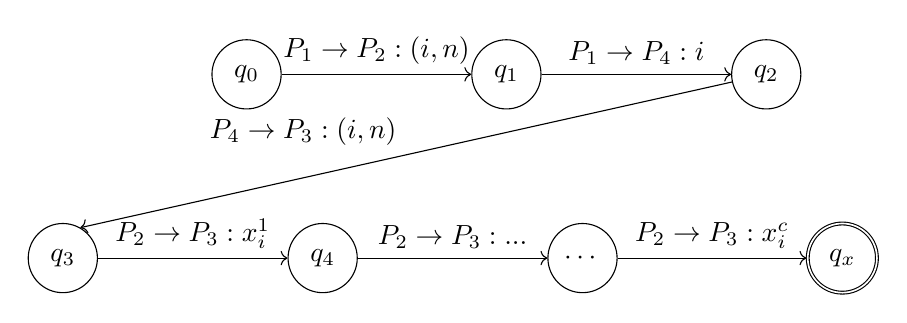
\begin{tikzpicture}[->, node distance=33mm, on grid, auto]
  \node[state] (q0) {$q_0$};
  \node[state] (q1) [right=of q0] {$q_1$};
  \node[state] (q2) [right=of q1] {$q_2$};
  \node[state] (q3) [below left=of q0] {$q_3$};
  \node[state] (q4) [right=of q3] {$q_4$};
  \node[state] (q5) [right=of q4] {$\cdots$};
  \node[state,accepting] (q6) [right=of q5] {$q_x$};

  \path (q0) edge[] node[above] {$P_1\to P_2:(i,n)$} (q1);
  \path (q1) edge[] node[above] {$P_1\to P_4:i$} (q2);
  \path (q2) edge[] node[above left] {$P_4\to P_3:(i,n)$} (q3.60);
  \path (q3) edge[] node[above] {$P_2\to P_3:x_i^1$} (q4);
  \path (q4) edge[] node[above] {$P_2\to P_3:...$} (q5);
  \path (q5) edge[] node[above] {$P_2\to P_3:x_i^c$} (q6);
\end{tikzpicture}
\end{center}
\end{frame}


\begin{frame}{The global type $L^*$}
  \vspace{-1cm}
  \begin{center}
  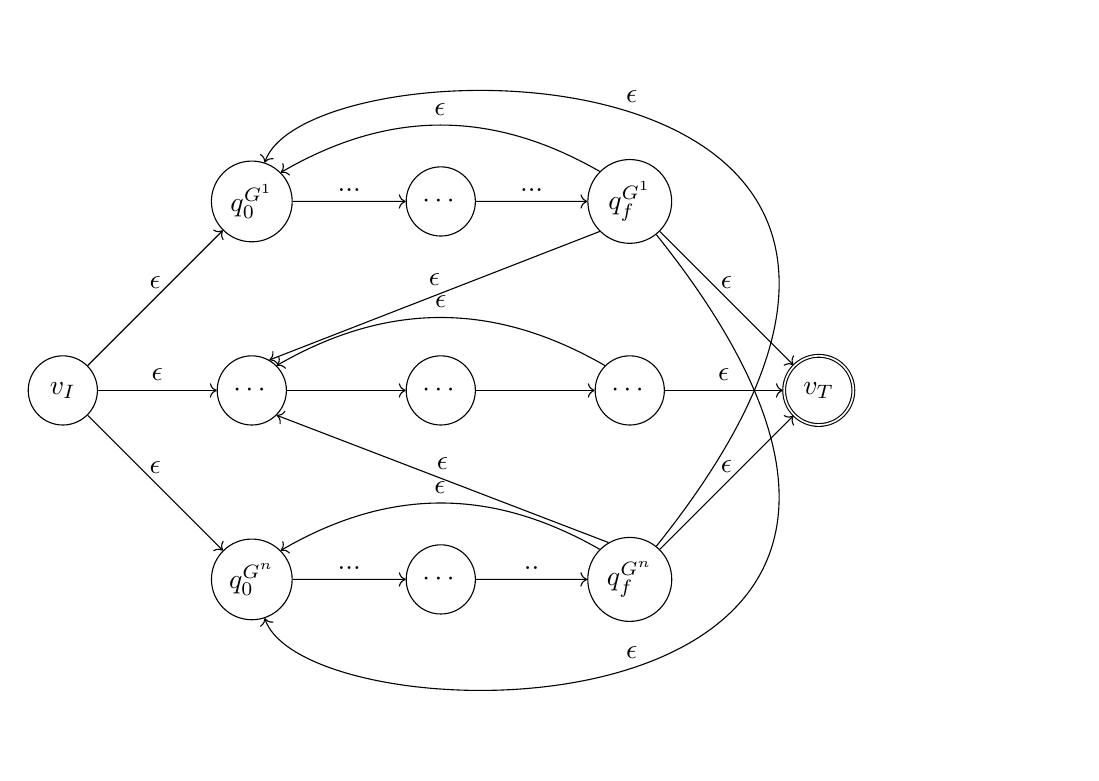
\begin{tikzpicture}[->, node distance=24mm,on grid,auto,scale=0.7]
		\node[state] (vI) {$v_I$};
		\node[state] (qI2) [right=of vI] {$\cdots$};
		\node[state] (qI1) [above=of qI2] {$q_0^{G^1}$};
		\node[state] (qI3) [below=of qI2] {$q_0^{G^n}$};
		\node[state] (qM1) [right=of qI1] {$\cdots$};
		\node[state] (qM2) [right=of qI2] {$\cdots$};
		\node[state] (qM3) [right=of qI3] {$\cdots$};
		\node[state] (qF1) [right=of qM1] {$q_f^{G^1}$};
		\node[state] (qF2) [right=of qM2] {$\cdots$};
		\node[state] (qF3) [right=of qM3] {$q_f^{G^n}$};
		\node[state,accepting] (vT) [right=of qF2] {$v_T$};

		\path (vI) edge[] node[above] {$\epsilon$} (qI1);
		\path (vI) edge[] node[above] {$\epsilon$} (qI2);
		\path (vI) edge[] node[above] {$\epsilon$} (qI3);
		\path (qI1) edge[] node[above] {...} (qM1);
		\path (qI2) edge[] node[above] {} (qM2);
		\path (qI3) edge[] node[above] {...} (qM3);
		\path (qM1) edge[] node[above] {...} (qF1);
		\path (qM2) edge[] node[above] {} (qF2);
		\path (qM3) edge[] node[above] {..} (qF3);
		\path (qF1) edge[] node[above] {$\epsilon$} (vT);
		\path (qF2) edge[] node[above] {$\epsilon$} (vT);
		\path (qF3) edge[] node[above] {$\epsilon$} (vT);
		
		\draw (qF1.135) to [bend right=30] node[above] {$\epsilon$} (qI1.45);
		\draw (qF2.135) to [bend right=30] node[above] {$\epsilon$} (qI2.45);
		\draw (qF3.135) to [bend right=30] node[above] {$\epsilon$} (qI3.45);

		\draw (qF1.225) to node[above] {$\epsilon$} (qI2.60);
		\draw (qF3.120) to node[above] {$\epsilon$} (qI2.315);
		
		\draw (qF3) .. controls +(8,10) and +(1,3) .. node[midway,above] {$\epsilon$} (qI1);
		\draw (qF1) ..  controls +(8,-10) and +(1,-3) .. node[midway,above] {$\epsilon$} (qI3);
	\end{tikzpicture}
  \end{center}
\end{frame}

\end{document}
